\section{A subcubic realization of the affine blocks}
\label{graph:section}

We now encode the block data by graphs of maximum degree three while
meeting the two hypotheses of \Cref{prop:game-reduction}.
We use the same affine blocks as in the general realization, but replace
the valuation graph and its private leaves by a different graph. Every
new vertex must still belong to just one block, and its local map must
depend only on that block's offset. We prove these properties together
with reached-history recognition; no generic degree-reduction theorem
or unrestricted-degree hardness theorem supplies this step.
Throughout this section take \(r\ge8\), so \(K=r+1\ge9\).

Write \(N=\abs{\cB}\).  We use the following conclusions of
\Cref{lem:block-fibers}.  A block \(B\) has a set \(\cR(B)\) of at most four
readout names, each with its specified one- or two-dimensional binary
value space.  The total number \(a_B\) of scalar coordinates is at most
six.  Its legal valuation sets satisfy
\[
  \cZ_B^0\text{ is a vector space},\qquad
  \cZ_B^1=\cZ_B^0+\xi
       \quad\text{for every }\xi\in\cZ_B^1,
\]
and both sets are nonempty.  Their projections onto any one named
readout are full.  The coordinates of a name have the same prescribed
order at every block that contains that name.  For a valuation \(z\)
and a name \(\rho\in\cR(B)\), write \(z|_\rho\) for its value on that
readout.

\Needspace{5\baselineskip}
\begin{proposition}[Subcubic realization]
\label{prop:subcubic-realization}
From the block data one can construct graphs \(X^0,X^1\), with
partitions
\[
  V(X^\eps)=\coprod_{B\in\cB}V_B^\eps
  \qquad(\eps\in\{0,1\}),
\]
having the following properties.
\begin{enumerate}
\item
Both graphs are finite, simple, connected, uncolored, and of maximum
degree at most three.  They have the same positive order.
Their orders are \(O(N^4)\), and the construction is polynomial in the
size of the explicitly listed block data.
\item
For each \(z\in\cZ_B^\eps\), the part \(V_B^\eps\) contains a specified
triangle \(T_B^\eps(z)\).  These triangles are pairwise disjoint.
For every \(\xi_B\in\cZ_B^1\), there is a fixed bijection
\[
  \Psi_{B,\xi_B}:V_B^0\longrightarrow V_B^1
\]
depending only on \(B,\xi_B\), and the constructed graphs.  It sends
\(T_B^0(z)\) onto \(T_B^1(z+\xi_B)\).
\par\Needspace{7\baselineskip}
If \(U\subseteq\cB\) and the offsets
\((\xi_B)_{B\in U}\) agree on all names shared by blocks in \(U\), then
the following map is an isomorphism of induced subgraphs:
\[
 \coprod_{B\in U}\Psi_{B,\xi_B}:
 X^0\left[\bigcup_{B\in U}V_B^0\right]
 \longrightarrow
 X^1\left[\bigcup_{B\in U}V_B^1\right].
\]
\item
Fix a winning Duplicator strategy in the \(K\)-slot bijection game,
where \(K=r+1\ge9\).
At every reached history, a marked vertex in \(T_B^0(z)\) is paired
with a vertex in \(T_B^1(z')\) for a unique \(z'\in\cZ_B^1\).
If simultaneous marked vertices lie in \(T_B^0(z)\) and \(T_C^0(w)\),
where \(B\ne C\), then, for each
\(\rho\in\cR(B)\cap\cR(C)\),
\[
     z|_\rho=w|_\rho
     \quad\Longrightarrow\quad
     z'|_\rho=w'|_\rho .
\]
These conclusions hold even when all \(K\) slots are occupied.
\end{enumerate}
\end{proposition}

We construct the graphs and establish the proposition in stages.

\subsection{Channels, prefix forests, and a connected colored graph}

For every block \(B\), form an ordered list of \emph{channels}.
Its first member is channel \(0\), which specifies no readout.
For every other block \(C\ne B\) and every shared name
\(\rho\in\cR(B)\cap\cR(C)\), add a channel denoted
\(c_B(C,\rho)\).
The channels \(c_B(C,\rho)\) and \(c_C(B,\rho)\) are called
\emph{opposite}.  Their order is fixed by the block data and is the
same in both versions.

In each channel \(c\) choose an order of the \(a_B\) scalar coordinates,
again common to the two versions.  In a proper channel
\(c=c_B(C,\rho)\), the coordinates of \(\rho\), in their prescribed
order, must come first.  Let
\[
 q_{Bc}=
 \begin{cases}
  0,&c=0,\\
  \dim(\rho),&c=c_B(C,\rho).
 \end{cases}
\]
For a valuation \(z\), denote its length-\(h\) prefix in channel \(c\)'s
order by \(\pi_{Bc,h}(z)\).
We build a vertex-colored graph \(Y^\eps\).
All vertex positions in the following list are distinct.

\begin{enumerate}
\item
\textbf{Spines.}
For every channel \(c\) and legal valuation \(z\in\cZ_B^\eps\),
create a vertex \(s_{Bc}^\eps(z)\).
For consecutive channels \(c,c+1\), join
\(s_{Bc}^\eps(z)\) to \(s_{B,c+1}^\eps(z)\).
Thus each valuation has one path through the channel list.
Set
\[
                  s_B^\eps(z)=s_{B0}^\eps(z)
\]
and call this its distinguished vertex.
\item
\textbf{Prefix forests.}
For \(q_{Bc}\le h\le a_B\), and every prefix \(u\) of length \(h\)
that extends to a valuation in \(\cZ_B^\eps\), create a vertex
\(f_{Bc,h}^\eps(u)\).
For \(h>q_{Bc}\), join it to the vertex indexed by its truncation
to length \(h-1\).
These are rooted trees whose roots have level \(q_{Bc}\).
Join the leaf
\(f_{Bc,a_B}^\eps(\pi_{Bc,a_B}(z))\)
to \(s_{Bc}^\eps(z)\).
\item
\textbf{Anchors.}
Create an anchor \(\alpha_B^\eps\) and join it to
\(f_{B0,0}^\eps(\varnothing)\).
Join the anchors in a path through all blocks in a fixed order.
\item
\textbf{Equality matchings.}
For opposite proper channels specifying \(\rho\), join their roots
with the same value of \(\rho\).
Write \(c=c_B(C,\rho)\), \(c'=c_C(B,\rho)\), and
\(q=\dim(\rho)=q_{Bc}=q_{Cc'}\).
For each \(u\) in the value space of \(\rho\), join
\[
 f_{Bc,q}^\eps(u)
 \quad\text{to}\quad
 f_{Cc',q}^\eps(u).
\]
Full projection onto \(\rho\) ensures that both roots exist for every
\(u\), so this is a perfect matching of the two root sets.
\end{enumerate}

If \(q_{Bc}=a_B\), a root is also a leaf: it is one vertex, adjacent
to its spine vertex and its opposite root.
There is no additional copy or truncation edge in this case.

The \emph{sorts} are: one anchor sort for each block; one spine sort
for each block and channel; and one tree sort for each block, channel,
and level.  If there are \(s\) sorts, assign them the consecutive
integers \(1,\ldots,s\) in a fixed enumeration order, common to the
two versions.
Let \(\operatorname{col}(v)\) be the resulting color of a vertex.
In particular, different labels within a sort receive the same color.
Assign every vertex just constructed at \(B\) to its \emph{block part}.

\begin{lemma}
\label{graph:colored-promises}
Each \(Y^\eps\) is simple, connected, and has maximum degree at most
three.  Each block part is connected.  There are \(O(N^2)\) vertices
and \(O(N^2)\) sorts.
\end{lemma}

\begin{proof}
A spine vertex has at most two spine neighbors and one leaf neighbor.
A nonroot internal tree vertex has one parent and at most two children.
A nonleaf root has at most two children and one further neighbor:
its anchor in channel zero, or its matched opposite root in a proper
channel.  A leaf has its spine neighbor and either its parent or,
when it is also a root, its matched opposite root.
An anchor has its channel-zero root neighbor and at most two neighbors
on the anchor path.
Thus every degree is at most three.

All tree, spine, and anchor vertices occupy distinct positions.
A proper root belongs to just one channel and has just one matching
edge.  Its opposite root belongs to a different block.
The remaining edge types have their distinct indicated endpoints,
so no loop or multiple edge is introduced.

Every legal prefix has a full legal extension.
It therefore reaches a leaf, then the spine at that channel.
The spine path reaches channel zero at the same valuation, and the
channel-zero tree reaches the anchor.
This proves connectedness of each block part.
The anchor path joins all parts.

There are at most
\[
 N+\sum_{B\ne C}\abs{\cR(B)\cap\cR(C)}
 \le N+4N(N-1)
\]
channels in total.
A channel has at most \(2^6\) spine vertices and at most
\(\sum_{h=0}^6 2^h\) tree vertices.
It also has at most eight sorts: one spine sort and at most seven
tree-level sorts.  Adding the \(N\) anchors and anchor sorts proves
both estimates.
\end{proof}

\begin{lemma}[A walk tests a shared readout]
\label{graph:readout-walk}
For distinct blocks \(B,C\) and a shared name \(\rho\), there is a
fixed sequence of sorts such that
\(s_B^\eps(z)\) and \(s_C^\eps(w)\) are joined by a walk following
that sequence if and only if \(z|_\rho=w|_\rho\).
The sequence is common to both versions.
\end{lemma}

\begin{proof}
Starting at channel zero of \(B\), follow its spine to
\(c_B(C,\rho)\), then go to the leaf and ascend its tree to the root.
Cross the matching to the opposite root in \(C\).
Descend to a leaf, go to its spine, and follow the spine to channel
zero of \(C\).
Record the sort at every position of this route.
When a root is also a leaf it contributes just one position.
The route is illustrated in \Cref{graph:fig-readout-route}.

The sorts specify the block and channel throughout, and the level
of each tree vertex.  Every spine step preserves the full valuation.
The leaf is indexed by that valuation, and truncation to the root
retains exactly the coordinates of \(\rho\).
The prescribed step to the opposite root can only use the matching
of equal values.  A descent on the other side extends that same root
value, and its subsequent spine steps preserve the chosen extension.
Consequently every walk with the specified sorts has equal endpoint
readouts.  Conversely, when the endpoint readouts agree, their two
prefix paths reach a matched pair of roots and give the required walk.
\end{proof}

\begin{figure}[tb]
\centering
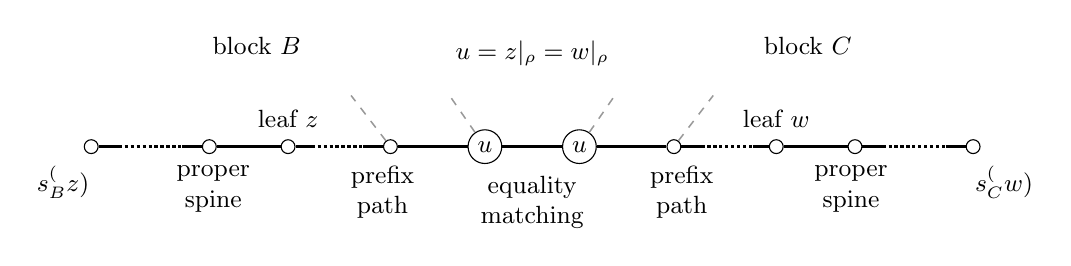
\begin{tikzpicture}[
  x=1cm,y=1cm,font=\small,
  vertex/.style={circle,draw,fill=white,inner sep=0pt,minimum size=5pt},
  root/.style={circle,draw,fill=white,inner sep=2pt},
  route/.style={line width=1.15pt},
  possible/.style={line width=.55pt,black!40,dashed}
]
  \node[vertex] (sB) at (-5.6,0) {};
  \node[vertex] (cB) at (-4.1,0) {};
  \node[vertex] (lB) at (-3.1,0) {};
  \node[vertex] (pB) at (-1.8,0) {};
  \node[root] (rB) at (-.6,0) {\(u\)};
  \node[root] (rC) at (.6,0) {\(u\)};
  \node[vertex] (pC) at (1.8,0) {};
  \node[vertex] (lC) at (3.1,0) {};
  \node[vertex] (cC) at (4.1,0) {};
  \node[vertex] (sC) at (5.6,0) {};
  \draw[route] (sB)--(-5.25,0) (-4.45,0)--(cB)--(lB);
  \draw[route,densely dotted] (-5.25,0)--(-4.45,0);
  \draw[route] (lB)--(-2.8,0) (-2.15,0)--(pB)--(rB);
  \draw[route,densely dotted] (-2.8,0)--(-2.15,0);
  \draw[route] (rB)--(rC)--(pC)--(2.15,0) (2.8,0)--(lC)--(cC);
  \draw[route,densely dotted] (2.15,0)--(2.8,0);
  \draw[route] (cC)--(4.45,0) (5.25,0)--(sC);
  \draw[route,densely dotted] (4.45,0)--(5.25,0);
  \draw[possible]
    (rB)--(-1.05,.65)
    (pB)--(-2.3,.65)
    (rC)--(1.05,.65)
    (pC)--(2.3,.65);
  \node[above] at (-3.5,1.05) {block \(B\)};
  \node[above] at (3.5,1.05) {block \(C\)};
  \node[below,anchor=north east] at (-5.5,-.12) {\(s_B^\eps(z)\)};
  \node[below,align=center] at (-4.05,-.12) {proper\\spine};
  \node[above] at (-3.1,.12) {leaf \(z\)};
  \node[below,align=center] at (-1.9,-.12) {prefix\\path};
  \node[below,align=center] at (1.9,-.12) {prefix\\path};
  \node[above] at (3.1,.12) {leaf \(w\)};
  \node[below,align=center] at (4.05,-.12) {proper\\spine};
  \node[below,anchor=north west] at (5.5,-.12) {\(s_C^\eps(w)\)};
  \node[below,align=center] at (0,-.25) {equality\\matching};
  \node[above] at (0,.9) {\(u=z|_\rho=w|_\rho\)};
\end{tikzpicture}
\caption{The walk that tests a shared readout \(\rho\).
The selected route follows a valuation's spine to the proper channel,
ascends its prefix tree to the root indexed by \(u\), crosses the
equality matching, and follows the opposite route to the other
distinguished vertex.
Dotted portions abbreviate intervening spine channels or tree levels.
Light dashed branches indicate possible additional legal prefixes;
the forests contain only prefixes with legal extensions and need not
be full binary trees.
A root and leaf coincide when their two levels agree.
Labels and line styles explain the diagram, without adding relations
to the colored graph.}
\label{graph:fig-readout-route}
\end{figure}


\Needspace{14\baselineskip}
\subsection{Translations that use one block offset}

\begin{lemma}[Colored block translations]
\label{graph:colored-translations}
Every \(\xi_B\in\cZ_B^1\) determines a color-preserving isomorphism
between the block parts of \(B\) in \(Y^0,Y^1\).
It fixes the anchor, sends
\[
 s_{Bc}^0(z)\longmapsto s_{Bc}^1(z+\xi_B),
 \qquad
 f_{Bc,h}^0(u)\longmapsto
 f_{Bc,h}^1\bigl(u+\pi_{Bc,h}(\xi_B)\bigr),
\]
and depends on no other block's offset.
On a union of parts, these maps form an induced-subgraph
isomorphism whenever the chosen offsets agree on shared names.
\end{lemma}

\begin{proof}
Translation by \(\xi_B\) bijects \(\cZ_B^0\) with \(\cZ_B^1\).
Its effect on a prefix depends only on that prefix and commutes with
truncation.  The displayed maps therefore give bijections at every
sort, preserving the tree, leaf-to-spine, and consecutive-channel
edges and their nonedges.
The empty prefix is fixed, so the anchor edge is preserved.

The only edges between parts are anchor-path edges and root-matching
edges.  Anchors are fixed individually.
For a root matching on \(\rho\), roots with values \(u,v\) are
adjacent exactly when \(u=v\).
If both block offsets have the same restriction \(d\) to \(\rho\),
then
\[
                       u=v\quad\Longleftrightarrow\quad u+d=v+d.
\]
This preserves both adjacency and nonadjacency across that matching.
Different channels stay different channels, so no other cross-part
adjacency can arise.
\end{proof}

\subsection{Removing the sort colors}

At each vertex \(v\) of \(Y^\eps\), assign its incident edges injectively
to ports \(1,2,3\), in any fixed construction order.
Replace \(v\) by a triangle with vertices
\[
                       t(v,1),\ t(v,2),\ t(v,3).
\]
For each \(j\), create a connector \(b(v,j)\) adjacent to \(t(v,j)\).
Attach a private path of length \(\operatorname{col}(v)\) to this
connector, with the connector as the path's initial vertex.
All other vertices on this path are new.
For an edge \(vw\) of \(Y^\eps\) assigned to ports \(j,j'\), add the
edge \(b(v,j)b(w,j')\).
No other edges or colors are retained.
Call the resulting uncolored graph \(X^\eps\).
The replacement gadget is shown in \Cref{graph:fig-uncoloring}.

Every new vertex made at \(v\) belongs to \(v\)'s block part.
In particular, the two endpoints of an edge between different blocks
belong to their respective blocks.
Denote these parts by \(V_B^\eps\).
The triangle replacing \(s_B^\eps(z)\) is denoted \(T_B^\eps(z)\).

\begin{figure}[tb]
\centering
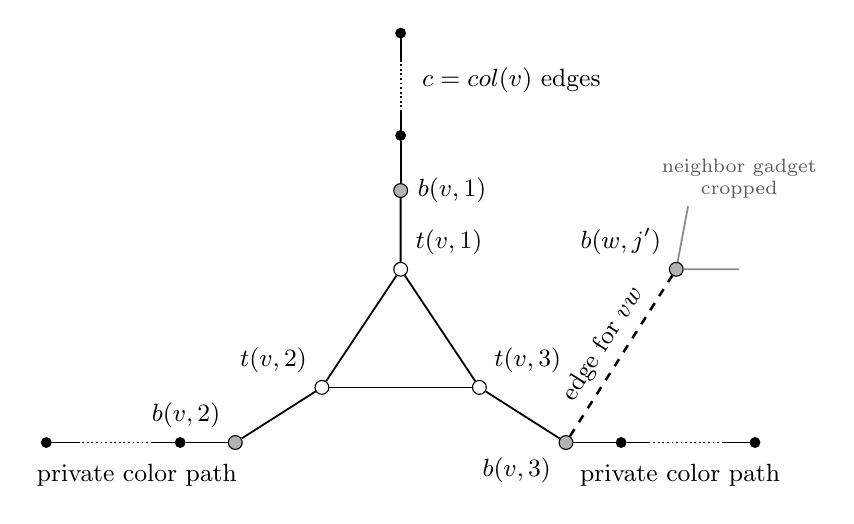
\begin{tikzpicture}[
  x=1cm,y=1cm,
  font=\small,
  vertex/.style={
    circle,draw,fill=white,inner sep=0pt,minimum size=5pt
  },
  connector/.style={vertex,fill=black!30},
  pathvertex/.style={vertex,fill=black,minimum size=3.5pt},
  graph edge/.style={line width=.65pt},
  external edge/.style={
    graph edge,dashed,line width=.9pt
  }
]
  \node[vertex,label=above right:{$t(v,1)$}] (t1) at (0,1) {};
  \node[vertex,label=above left:{$t(v,2)$}] (t2) at (-1,-.5) {};
  \node[vertex,label=above right:{$t(v,3)$}] (t3) at (1,-.5) {};
  \draw[graph edge] (t1)--(t2);
  \draw[graph edge] (t2)--(t3);
  \draw[graph edge] (t3)--(t1);
  \node[connector,label=right:{$b(v,1)$}] (b1) at (0,2) {};
  \node[connector,label=above left:{$b(v,2)$}]
    (b2) at (-2.1,-1.2) {};
  \node[connector,label=below left:{$b(v,3)$}]
    (b3) at (2.1,-1.2) {};
  \draw[graph edge] (t1)--(b1) (t2)--(b2) (t3)--(b3);

  \node[pathvertex] (p11) at (0,2.7) {};
  \node[pathvertex] (p1c) at (0,4) {};
  \draw[graph edge] (b1)--(p11)--(0,3);
  \draw[graph edge,densely dotted] (0,3)--(0,3.65);
  \draw[graph edge] (0,3.65)--(p1c);
  \node[right] at (.15,3.4)
    {$c=\operatorname{col}(v)$ edges};

  \node[pathvertex] (p21) at (-2.8,-1.2) {};
  \node[pathvertex] (p2c) at (-4.5,-1.2) {};
  \draw[graph edge] (b2)--(p21)--(-3.15,-1.2);
  \draw[graph edge,densely dotted]
    (-3.15,-1.2)--(-4.1,-1.2);
  \draw[graph edge] (-4.1,-1.2)--(p2c);
  \node[pathvertex] (p31) at (2.8,-1.2) {};
  \node[pathvertex] (p3c) at (4.5,-1.2) {};
  \draw[graph edge] (b3)--(p31)--(3.15,-1.2);
  \draw[graph edge,densely dotted]
    (3.15,-1.2)--(4.1,-1.2);
  \draw[graph edge] (4.1,-1.2)--(p3c);
  \node[below] at (-3.35,-1.35) {private color path};
  \node[below] at (3.55,-1.35) {private color path};

  \node[connector,label=above left:{$b(w,j')$}]
    (bw) at (3.5,1) {};
  \draw[external edge]
    (b3)--node[midway,above,sloped] {edge for \(vw\)} (bw);
  \draw[graph edge,black!45]
    (bw)--(3.65,1.8)
    (bw)--(4.3,1);
  \node[font=\scriptsize,black!65,align=center]
    at (4.3,2.15) {neighbor gadget\\cropped};
\end{tikzpicture}
\caption{The uncoloring gadget at a vertex \(v\).
Each triangle member has its own connector and each connector
has a private path of exactly \(c=\operatorname{col}(v)\) edges.
Dotted portions abbreviate path interiors; for \(c=1\), each private
path is a single pendant edge.
The dashed edge represents an original edge \(vw\) attached at its
chosen ports.  In this schematic example \(b(v,3)\) uses its external
port, while \(b(v,1)\) and \(b(v,2)\) do not.
The neighboring gadget is cropped, with its connector's other two
incidences shown as short stubs.
Shading and line styles explain the construction and are not graph
colors or additional relations.}
\label{graph:fig-uncoloring}
\end{figure}


\begin{lemma}[Uncolored promises and local lifts]
\label{graph:uncolored-lifts}
The graphs \(X^\eps\) are simple, connected, uncolored, and of maximum
degree at most three.  They have the same positive order, of size
\(O(N^4)\).
Each colored block translation in \Cref{graph:colored-translations}
has a fixed lift \(\Psi_{B,\xi_B}:V_B^0\to V_B^1\), depending only
on that offset, satisfying the induced-isomorphism assertion of
\Cref{prop:subcubic-realization}.
\end{lemma}

\begin{proof}
Every triangle member has degree three.
A connector has its triangle neighbor and its first path neighbor,
and, precisely when its port is used, one external connector neighbor.
Its degree is therefore two or three.
All other path vertices have degree at most two.
The edge lists introduce neither loops nor repeated edges.
Each replacement is connected, and replacements are joined exactly
along the original graph's edges; hence \(X^\eps\) is connected.
There is at least one block, each with nonempty legal valuations,
so the order is positive.

Fix a block and offset, and write \(v'\) for the image of a vertex
\(v\) under its colored block translation.
Define a permutation of the three ports at \(v\) to those at \(v'\)
as follows.
\begin{enumerate}
\item
A port used by an edge within the block goes to the port used by the
image of that edge under the colored translation.
\item
At an anchor, a port used by an external anchor-path edge goes to the
port for the anchor-path edge toward the same other block.
\item
At a proper-channel root, the port used by its edge to the opposite
root goes to the port for the unique such edge at its image root.
\item
The unused ports are matched in their fixed numerical orders.
\end{enumerate}
These prescriptions are disjoint and exhaustive.
Internal incidences are bijected by a within-block isomorphism.
Each anchor retains the same external anchor incidences, and each
proper root has exactly one external incidence at both source and
image.  Thus the unused port counts also agree, and the prescriptions
indeed give a permutation.
Crucially, the third prescription does not require the neighboring
block's offset.

Using this port permutation, map triangle members to triangle members,
connectors to connectors, and private paths in order to their
corresponding private paths.  The colors of \(v,v'\) agree, so the
path lengths agree.  This gives a bijection
\(\Psi_{B,\xi_B}\) of the block parts, with the asserted action on the
distinguished triangles.

For compatible offsets on a union of blocks, every internal edge and
every anchor edge is carried to the edge prescribed by its endpoint
port permutations.
For an equality matching, the root values are shifted by the same
readout offset, so the equality condition is preserved in both
directions.  At its two endpoints the unique external ports are
exactly the ports used by that matching.
Unused ports remain unused, and all channels remain their own channels.
It follows that all edges and nonedges between replacements in the
union are preserved.  The maps inside the replacements are also
isomorphisms, proving the induced-subgraph assertion.
Edges leaving the union impose no condition on unchosen offsets.

For equal orders, choose an arbitrary legal offset separately at each
block.  The resulting bijections of disjoint parts give a bijection
of the two vertex sets; compatibility is not needed for this count.
Finally, if the number of sorts is \(s\), a colored vertex of color
\(c\) produces exactly \(6+3c\) vertices.
By \Cref{graph:colored-promises}, both \(s\) and \(\abs{V(Y^\eps)}\)
are \(O(N^2)\), giving the order bound \(O(N^4)\).
All enumerations use at most six-bit valuations and prefixes, explicit
block pairs and shared names, and paths of polynomial length.
They therefore implement the construction in polynomial time.
\end{proof}

\subsection{What a winning game must preserve}

To establish the decoding hypothesis of \Cref{prop:game-reduction},
we use the reached-history principle from \Cref{game:section}.
A hypothetical continuation may discard unrelated pairs to test the
retained pairs. If failure of an asserted property would let Spoiler
force a loss, that property must already hold at the original history.
The test need not return to that history or restore discarded answers.
Thus the tests below establish invariants even when all slots are occupied.

\begin{lemma}[Recognition under a winning strategy]
\label{lem:graph-recognition}
Let \(K\ge6\), and fix a winning strategy on \(X^0,X^1\).
At every reached history:
\begin{enumerate}
\item
Paired vertices have the same degree and agree as to whether they lie
in a triangle.
\item
A triangle member over \(v\in V(Y^0)\) is paired with a triangle
member over some \(v'\in V(Y^1)\) of the same sort.
\item
If two marked triangle members lie over adjacent vertices \(v,w\)
of \(Y^0\), their responses lie over adjacent vertices \(v',w'\)
of \(Y^1\).
\item
A marked member of \(T_B^0(z)\) has a unique decoded response
\(z'\in\cZ_B^1\), meaning that its response belongs to \(T_B^1(z')\).
For simultaneous marked members at distinct blocks, equality of any
shared readout implies equality of the decoded response readouts.
\end{enumerate}
The conclusions do not require a free slot at the history in question.
\end{lemma}

\begin{proof}
\emph{Degrees and triangles.}
Retain a paired vertex and request one further slot.
For every vertex Spoiler could choose, Duplicator's announced
bijection must preserve adjacency to the retained vertex.
The bijection therefore takes its neighbor set onto the other
neighbor set, proving degree equality with two slots.
To test membership in a triangle, retain the vertex and mark the two
other triangle members, using three slots.
The converse can be tested in the second graph: after a bijection is
announced, Spoiler can choose the preimage of any desired
second-graph vertex.  Partial isomorphism then proves triangle
membership in both directions.

The only triangles in \(X^\eps\) are the designated replacement
triangles.
Indeed, private path vertices cannot lie in a triangle; a connector
has only one triangle-vertex neighbor; and edges between connectors
form a matching, since each connector is a single port.
There are no other edges between replacements.
Thus a response to a triangle member lies in a unique replacement
triangle.

\emph{Sort recovery.}
Retain such a pair, and mark the connector attached to its
first-graph triangle member.
By triangle membership and adjacency, its response is the unique
nontriangle neighbor of the second-graph triangle member.
At a connector, the first private-path vertex is its unique neighbor
of degree below three.
The triangle member has degree three, and any connector reached
across an external connector edge has degree three because that port
is used.  This assertion also covers an unused connector and a
private path of length one.
Consequently a third mark forces the first private-path step.

Continue along the source path, retaining the previous and current
vertices and using a third slot for the next vertex.
Adjacency and inequality from the previous vertex force the forward
step in the target private path.
The original triangle mark can be discarded once the traversal has
started.
If the lengths differed, at their first discrepancy a terminal vertex
of degree one would be paired with an internal vertex of degree two.
The degree invariant excludes this.
The path lengths, and therefore the sort numbers, are equal.
All assertions used during this test are invariants of reached
winning histories, established by their own alternative continuations.

\emph{Underlying adjacency.}
Retain the two marked triangle representatives over \(v,w\), and
also mark the actual triangle ports used by \(vw\) and the two
connectors attached to those ports.  This requires at most six slots.
An actual port may already be the representative; duplicate marking
is allowed, or its extra mark may be omitted.
Its response lies in the same triangle as its original
representative, by equality in the coincident case and by adjacency
and triangle membership otherwise.
Each connector response must be the unique nontriangle neighbor of
its port response.  The two connectors are adjacent, so their
underlying auxiliary vertices are adjacent in \(Y^1\).
The two response representatives cannot belong to one triangle:
the source representatives are distinct and nonadjacent, whereas
distinct members of one triangle are adjacent.

\emph{Distinguished vertices and shared readouts.}
Sort recovery sends a triangle over a channel-zero spine vertex
of block \(B\) to a triangle over another channel-zero spine vertex
of that same block.  The legal valuation indexing this vertex gives
the unique decoded response.

Suppose now that the two source valuations at distinct blocks agree
on a shared readout.
Their distinguished vertices admit the sort-prescribed walk from
\Cref{graph:readout-walk}.
First discard all marked pairs except these two endpoint pairs.
Mark triangle members over the intermediate vertices successively,
always retaining both endpoints and at most two consecutive
intermediate pairs.  Four slots suffice.
Sort recovery gives the required sorts of all response vertices.
Underlying adjacency, applied to each consecutive pair when both are
marked, shows that the responses trace a walk of precisely the
prescribed sorts.
\Cref{graph:readout-walk} now forces equality of the response readouts.

The four walk slots need not be supplemented by six adjacency-test
slots.  Underlying adjacency is already an invariant of every reached
winning history: its proof may discard the unrelated endpoint pairs
in a different continuation.  Similarly, the unary tests need not
retain the other walk marks.
The largest simultaneous test uses six slots, and the conclusion
about the retained endpoints therefore holds already at the original
history, regardless of its occupancy.
\end{proof}

\Needspace{8\baselineskip}
\begin{proof}[Proof of \Cref{prop:subcubic-realization}]
The graph promises, equal orders, size bound, local lifts, and
compatible-union isomorphisms are
\Cref{graph:colored-promises,graph:uncolored-lifts}.
The distinguished triangles have the stated indexing by construction.
Since \(K=r+1\ge9\), \Cref{lem:graph-recognition} supplies the
decoding and shared-readout invariants.
\end{proof}


\begin{corollary}[Correctness of the subcubic realization]
\label{cor:subcubic-game}
For every product scalar-image instance at address length \(r\ge8\),
its connected subcubic realization satisfies
\[
 \text{the instance is consistent}\quad\Longleftrightarrow\quad
 X^0\equiv_r X^1.
\]
\end{corollary}
\begin{proof}
Use \(\mathcal D_B^\eps(z)=T_B^\eps(z)\) in
\Cref{prop:game-reduction}. The block maps and decoding properties are
exactly those proved in \Cref{prop:subcubic-realization}; its parameter
condition holds because \(r\ge8\).
\end{proof}
